\documentclass[11pt]{article}
\usepackage[margin=1in]{geometry}
\usepackage{amsmath,amssymb,amsthm,mathtools}
\usepackage{booktabs}
\usepackage{graphicx}
\usepackage{microtype}
\usepackage{enumitem}
\usepackage[hidelinks]{hyperref}
\usepackage[nameinlink,capitalise]{cleveref}

\newtheorem{theorem}{Theorem}[section]
\newtheorem{proposition}[theorem]{Proposition}
\newtheorem{lemma}[theorem]{Lemma}
\newtheorem{corollary}[theorem]{Corollary}
\theoremstyle{definition}
\newtheorem{definition}[theorem]{Definition}
\newtheorem{remark}[theorem]{Remark}

\newcommand{\Q}{\mathbb Q}
\newcommand{\Z}{\mathbb Z}
\newcommand{\R}{\mathbb R}
\newcommand{\OK}{\mathcal O_K}
\DeclareMathOperator{\Nm}{N}
\DeclareMathOperator{\disc}{disc}

\title{\textbf{A Norm-Coset Reduction and a Certified Exceptional Interval\\in a Cyclic Cubic Field}}
\author{Ryan Gomez}
\date{October 2, 2026}

\begin{document}
\maketitle

\begin{abstract}
Let $K=\Q(\theta)$, where $\theta^3-3\theta-1=0$, and order the three real embeddings so that $\sigma_0(\theta)$ is the positive root.  For $H>0$ we study
\[
M(H)=\min_{0\ne\alpha\in\OK,\ |\sigma_0(\alpha)|\le H}
\max\bigl(|\sigma_1(\alpha)|,|\sigma_2(\alpha)|\bigr).
\]
We prove two results.  First, every optimizer has absolute norm $1$ or $3$.  Equivalently, every optimizer belongs to one of the two multiplicative layers
\[
\OK^\times\qquad\text{or}\qquad (\theta-1)\OK^\times.
\]
The proof combines a rigorous log-lattice covering certificate with the arithmetic gap in possible small norms.
Second, we give a globally complete exact certificate for the nonunit
\[
\beta=1+5\theta+3\theta^2=(\theta-1)(\theta+1)^3.
\]
If $L$ is the largest root of $x^3-21x^2+3$ and $U$ is the largest root of
$x^3-24x^2+3x+1$, then
\[
L\le H<U\quad\Longrightarrow\quad
\operatorname*{argmin} M(H)=\{\pm\beta\}.
\]
At $H=U$ the unique minimizers up to sign are
$\gamma=2+6\theta+3\theta^2=(\theta+1)^3$.
The key completeness step proves that any optimizer in this transition window must lie among exactly $454$ coefficient triples; the accompanying verifier checks all comparisons with rational interval arithmetic and uses no floating-point decisions.
\end{abstract}

\section{The optimization problem}
Let
\[
f(x)=x^3-3x-1,
\qquad K=\Q(\theta),\quad f(\theta)=0.
\]
The polynomial is irreducible by the rational-root test and has discriminant $81$, so $K$ is a cyclic totally real cubic field.  Write its real roots as
\[
r_1<r_2<r_0,
\]
where
\[
\begin{aligned}
r_0&=1.879385241571816\ldots,\\
r_1&=-1.532088886237956\ldots,\\
r_2&=-0.347296355333861\ldots,
\end{aligned}
\]
and set $\sigma_i(\theta)=r_i$.

For $\alpha\ne0$, define
\[
F(\alpha)=\max\bigl(|\sigma_1(\alpha)|,|\sigma_2(\alpha)|\bigr).
\]
At height $H>0$ we minimize $F$ subject to a one-sided archimedean constraint:
\begin{equation}\label{eq:M}
M(H)=\min_{0\ne\alpha\in\OK,\ |\sigma_0(\alpha)|\le H}F(\alpha).
\end{equation}
The asymmetric role of $\sigma_0$ is deliberate.  It makes the problem different from the usual symmetric height minimization and produces discrete transitions between unit and nonunit layers.

\subsection{The full ring of integers}
We will use the power basis without qualification.

\begin{lemma}\label{lem:ring}
$\OK=\Z[\theta]$.
\end{lemma}
\begin{proof}
The discriminant of the order $\Z[\theta]$ is $81$.  If
$I=[\OK:\Z[\theta]]$, then $I^2\mid81$ and
$\disc(K)=81/I^2$.  If $I>1$, then $\disc(K)$ would be $9$ or $1$.
Minkowski's discriminant bound for a totally real cubic field gives
\[
\sqrt{|\disc(K)|}\ge \frac{3^3}{3!}=\frac92,
\]
so $|\disc(K)|>20$.  Hence $I=1$.
\end{proof}

The Minkowski embedding of $\OK$ is a lattice in $\R^3$.  Once one feasible point is known, the intersection of that lattice with a bounded box is finite, so the minimum in \eqref{eq:M} exists.  A uniform feasible unit will be supplied below.

\section{A global norm-coset reduction}
For $\alpha\in K^\times$ put
\[
p(\alpha)=\log|\sigma_0(\alpha)|,
\qquad
q(\alpha)=\frac{\log|\sigma_1(\alpha)|-\log|\sigma_2(\alpha)|}{2}.
\]
If $u$ is a unit, then the product formula gives
\begin{equation}\label{eq:unit-objective}
\log F(u)=-\frac{p(u)}2+|q(u)|.
\end{equation}
Thus for $B=\log H$ and a feasible unit $p(u)\le B$,
\begin{equation}\label{eq:gauge}
\log\bigl(F(u)\sqrt H\bigr)
=\frac{B-p(u)}2+|q(u)|.
\end{equation}
This turns the search for a uniformly good unit into a covering problem in two dimensions.

Let
\[
\varepsilon=\theta+1.
\]
Both $\theta$ and $\varepsilon$ are units.  Their $(p,q)$ vectors are approximately
\[
\begin{aligned}
v_1&=(0.630944724202046,\ 0.742104451473912),\\
v_2&=(1.057576813574935,\ -0.102156317414579).
\end{aligned}
\]
Their determinant is $-0.849287450646\ldots\ne0$, so they generate a rank-two sublattice $\Lambda_0$ of the unit log lattice.

For $R>0$, define the one-sided triangle
\[
T_R=\{(x,y):x\ge0,\ x/2+|y|\le R\}.
\]

\begin{lemma}[Certified unit cover]\label{lem:cover}
For every $z\in\R^2$ there exists $\lambda\in\Lambda_0$ such that
\[
z-\lambda\in T_{9/10}.
\]
Consequently, for every $H>0$ there is a unit $u\in\langle\theta,\varepsilon\rangle$ satisfying
\begin{equation}\label{eq:unit-cover-bound}
|\sigma_0(u)|\le H,
\qquad
F(u)\le \frac{e^{9/10}}{\sqrt H}.
\end{equation}
\end{lemma}

\begin{proof}
Reduce $z$ modulo $\Lambda_0$ to the centered fundamental parallelogram
\[
P=\{s v_1+t v_2:-\tfrac12\le s,t\le\tfrac12\}.
\]
It is enough to prove that for every $e\in P$, one of
\[
e,\quad e+v_1,\quad e+v_2,\quad e+v_1+v_2
\]
lies in $T_{9/10}$.

The accompanying verifier proves this by exact interval arithmetic.  It first isolates the three roots of $f$ in rational intervals of width $10^{-30}$.  Logarithms are then enclosed by the exact series
\[
\log x=2\sum_{k=0}^{N}\frac{z^{2k+1}}{2k+1}+R_N,
\qquad z=\frac{x-1}{x+1},
\]
with a rational geometric bound on $R_N$.  The square
$[-\tfrac12,\tfrac12]^2$ in $(s,t)$ coordinates is divided into $16^2$ rational rectangles.  On every cell, interval evaluation certifies one of the four displayed shifts.  The largest cell-wise upper bound obtained is
\[
0.892330436453852\ldots<0.9.
\]
No floating-point value is used in a pass/fail decision.  Applying the result to $z=(\log H,0)$ and using \eqref{eq:gauge} gives \eqref{eq:unit-cover-bound}.
\end{proof}

We next identify a gap in the possible small absolute norms.

\begin{lemma}[Small-norm gap]\label{lem:norm-gap}
If $0\ne\alpha\in\OK$, then
\[
|\Nm(\alpha)|\in\{1,3\}\quad\text{or}\quad |\Nm(\alpha)|\ge8.
\]
\end{lemma}
\begin{proof}
Modulo each of $2,5,7$, the cubic $f$ has no root and is therefore irreducible.  By \cref{lem:ring}, Dedekind factorization applies directly, so each of $2,5,7$ is inert.  If one of these primes divides $\Nm(\alpha)$, then the corresponding prime ideal divides $(\alpha)$; inertness forces $(p)\mid(\alpha)$ and hence $p^3\mid\Nm(\alpha)$.  Therefore absolute norms $2,4,5,6,7$ cannot occur.  Since norms of nonzero algebraic integers are nonzero rational integers, the conclusion follows.
\end{proof}

\begin{theorem}[Global norm-coset reduction]\label{thm:global-reduction}
For every $H>0$, every optimizer in \eqref{eq:M} has absolute norm $1$ or $3$.  More precisely,
\[
\operatorname*{argmin} M(H)
\subseteq
\OK^\times\cup(\theta-1)\OK^\times.
\]
\end{theorem}
\begin{proof}
For any feasible $\alpha$,
\[
|\Nm(\alpha)|
=|\sigma_0(\alpha)\sigma_1(\alpha)\sigma_2(\alpha)|
\le H F(\alpha)^2,
\]
so
\begin{equation}\label{eq:norm-lower}
F(\alpha)\ge\sqrt{\frac{|\Nm(\alpha)|}{H}}.
\end{equation}
By \cref{lem:cover}, a feasible unit satisfies
$F(u)\le e^{9/10}H^{-1/2}$.  On the other hand,
\[
\log\sqrt8=\frac32\log2>1>\frac9{10};
\]
for example $\log2=2(1/3+1/(3^3\cdot3)+\cdots)>2/3$.
Hence $e^{9/10}<\sqrt8$, and \eqref{eq:norm-lower} excludes every element with absolute norm at least $8$ from being optimal.  By \cref{lem:norm-gap}, an optimizer has absolute norm $1$ or $3$.

It remains to identify the norm-$3$ layer.  Set $\delta=\theta-1$.  Then $\Nm(\delta)=3$, and from $f(\delta+1)=0$,
\[
\delta^3=3(1-\delta^2).
\]
Moreover
\[
1-\delta^2=\theta(2-\theta),
\qquad
(2-\theta)(\theta+1)^2=1,
\]
so $1-\delta^2$ is a unit.  Thus, as ideals,
\[
(3)=(\delta)^3.
\]
There is a unique prime ideal above $3$, namely $(\delta)$.  If $|\Nm(\alpha)|=3$, then $(\alpha)$ is a prime ideal of norm $3$, hence $(\alpha)=(\delta)$, and therefore $\alpha=\delta u$ for a unit $u$.
\end{proof}

\Cref{thm:global-reduction} is a structural statement: the global optimizer problem is exactly a competition between the unit lattice and one translated unit lattice.  It does not, by itself, determine every switching height.

\begin{figure}[t]
\centering
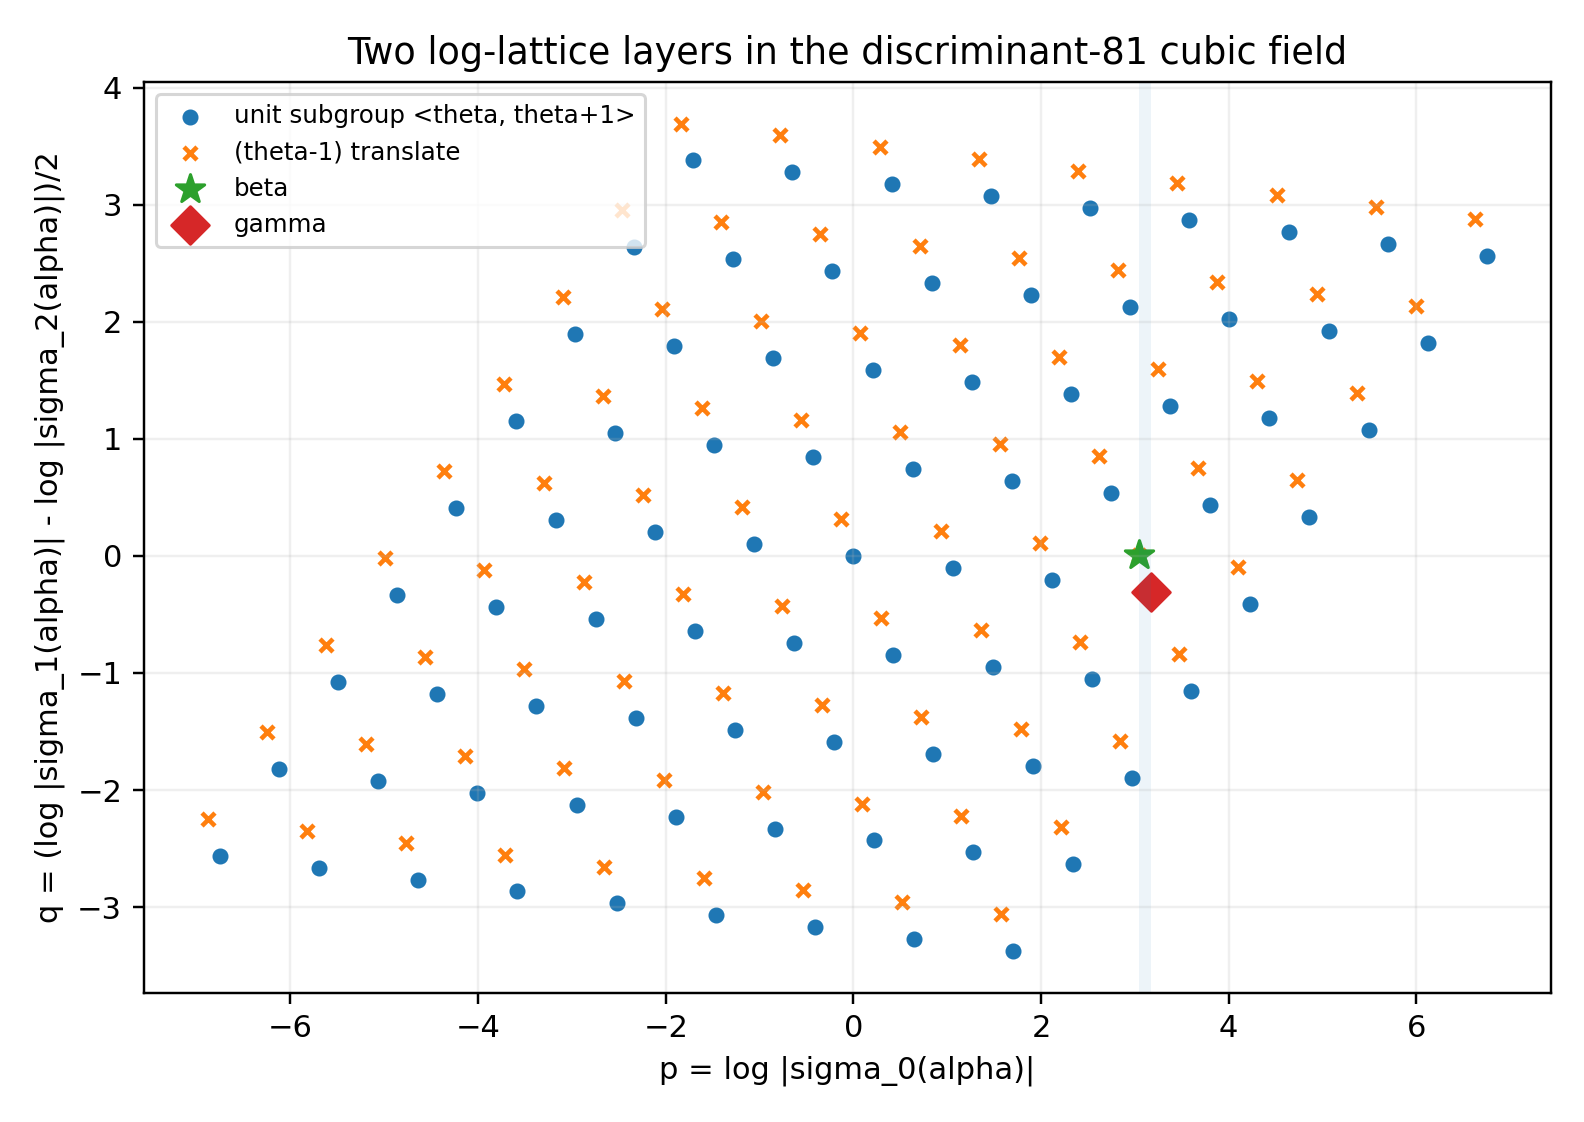
\includegraphics[width=0.84\textwidth]{log_lattice.png}
\caption{The subgroup generated by $\theta$ and $\theta+1$ in $(p,q)$ coordinates, together with the translate by $\theta-1$.  The highlighted points are $\beta=(\theta-1)(\theta+1)^3$ and $\gamma=(\theta+1)^3$.  The shaded vertical band marks $\log L\le p<\log U$.}
\label{fig:lattice}
\end{figure}

\section{The certified exceptional interval}
Define
\[
\beta=1+5\theta+3\theta^2=(\theta-1)(\theta+1)^3
\]
and
\[
\gamma=2+6\theta+3\theta^2=(\theta+1)^3.
\]
Their norms are
\[
\Nm(\beta)=-3,
\qquad
\Nm(\gamma)=-1,
\]
so $\beta$ is a nonunit and $\gamma$ is a unit.

Let
\[
P_\beta(x)=x^3-21x^2+3,
\qquad
P_\gamma(x)=x^3-24x^2+3x+1.
\]
Direct reduction modulo $\theta^3-3\theta-1$ verifies
$P_\beta(\beta)=P_\gamma(\gamma)=0$.  Let $L$ and $U$ denote the largest real roots of these polynomials.  Certified intervals are
\begin{align*}
20.993192866572952051755448676572
&<L<
20.993192866572952051755448676589,\\
23.872578108144768819863667231221
&<U<
23.872578108144768819863667231239.
\end{align*}
Under our ordering of embeddings,
\[
L=\sigma_0(\beta),\qquad U=\sigma_0(\gamma).
\]
Also set
\[
B=F(\beta),\qquad G=F(\gamma),
\]
with
\begin{align*}
0.381444634811801741086373255053
&<B<0.381444634811801741086373255068,\\
0.278066143281385509454744814816
&<G<0.278066143281385509454744814825.
\end{align*}
In particular $G<B$.

The finite certificate becomes global because a putative optimizer in this window has sharply bounded coefficients.

\begin{lemma}[Completeness of the 454-triple box]\label{lem:box}
Suppose $L\le H\le U$, and suppose $\alpha=a+b\theta+c\theta^2\in\OK$ satisfies
\[
|\sigma_0(\alpha)|\le U,
\qquad
F(\alpha)\le B.
\]
Then
\[
|a|\le2,\qquad |b|\le6,\qquad |c|\le3.
\]
\end{lemma}
\begin{proof}
Write $y_i=\sigma_i(\alpha)$.  Lagrange interpolation at the roots $r_i$ of $f$ gives, with $D_i=f'(r_i)=3r_i^2-3$,
\[
\begin{aligned}
c&=\sum_{i=0}^2\frac{y_i}{D_i},\\
b&=\sum_{i=0}^2\frac{r_i y_i}{D_i},\\
a&=\sum_{i=0}^2\frac{y_i}{r_iD_i}.
\end{aligned}
\]
Using $|y_0|\le U$ and $|y_1|,|y_2|\le B$, exact rational interval evaluation gives
\[
|a|<2.150102039486393,
\quad
|b|<6.101094622358899,
\quad
|c|<3.381632943042300.
\]
The coefficients are integers by \cref{lem:ring}, so the asserted integral bounds follow.
\end{proof}

There are exactly
\[
(2\cdot2+1)(2\cdot6+1)(2\cdot3+1)-1
=5\cdot13\cdot7-1=454
\]
nonzero triples in this box.

\begin{theorem}[Exact global exceptional interval]\label{thm:beta}
For every $H$ with
\[
L\le H<U,
\]
the unique minimizers up to sign are $\pm\beta$:
\[
\operatorname*{argmin} M(H)=\{\pm\beta\}.
\]
At the right endpoint,
\[
\operatorname*{argmin} M(U)=\{\pm\gamma\}.
\]
Consequently, $\beta$ is a global optimizer exactly on $[L,U)$, and every $H$ in this interval is exceptional in the sense that the optimizer is a nonunit.
\end{theorem}

\begin{proof}
Take $L\le H<U$.  The element $\beta$ is feasible, so $M(H)\le B$.  If $\alpha$ is any optimizer, then
\[
|\sigma_0(\alpha)|\le H<U,
\qquad
F(\alpha)\le B.
\]
By \cref{lem:box}, $\alpha$ lies in the 454-triple box.

The exact verifier evaluates every one of those triples on certified rational intervals for the three roots.  Among all candidates with
$|\sigma_0(\alpha)|<U$, the only two whose objective is at most $B$ are $\beta$ and $-\beta$; every other candidate has a rigorously separated lower objective bound greater than the rigorous upper bound for $B$.  This proves the first assertion.

At $H=U$, $\gamma$ is feasible and has objective $G<B$.  The same coefficient bound remains valid.  Exact enumeration shows that every one of the other 452 triples has objective strictly greater than $G$.  Hence the unique minimizers up to sign are $\pm\gamma$.

Below $L$, $\beta$ is infeasible.  At and above $U$, the permanently feasible unit $\gamma$ has strictly smaller objective.  Therefore the full optimizer interval of $\beta$ is exactly $[L,U)$.
\end{proof}

\begin{figure}[t]
\centering
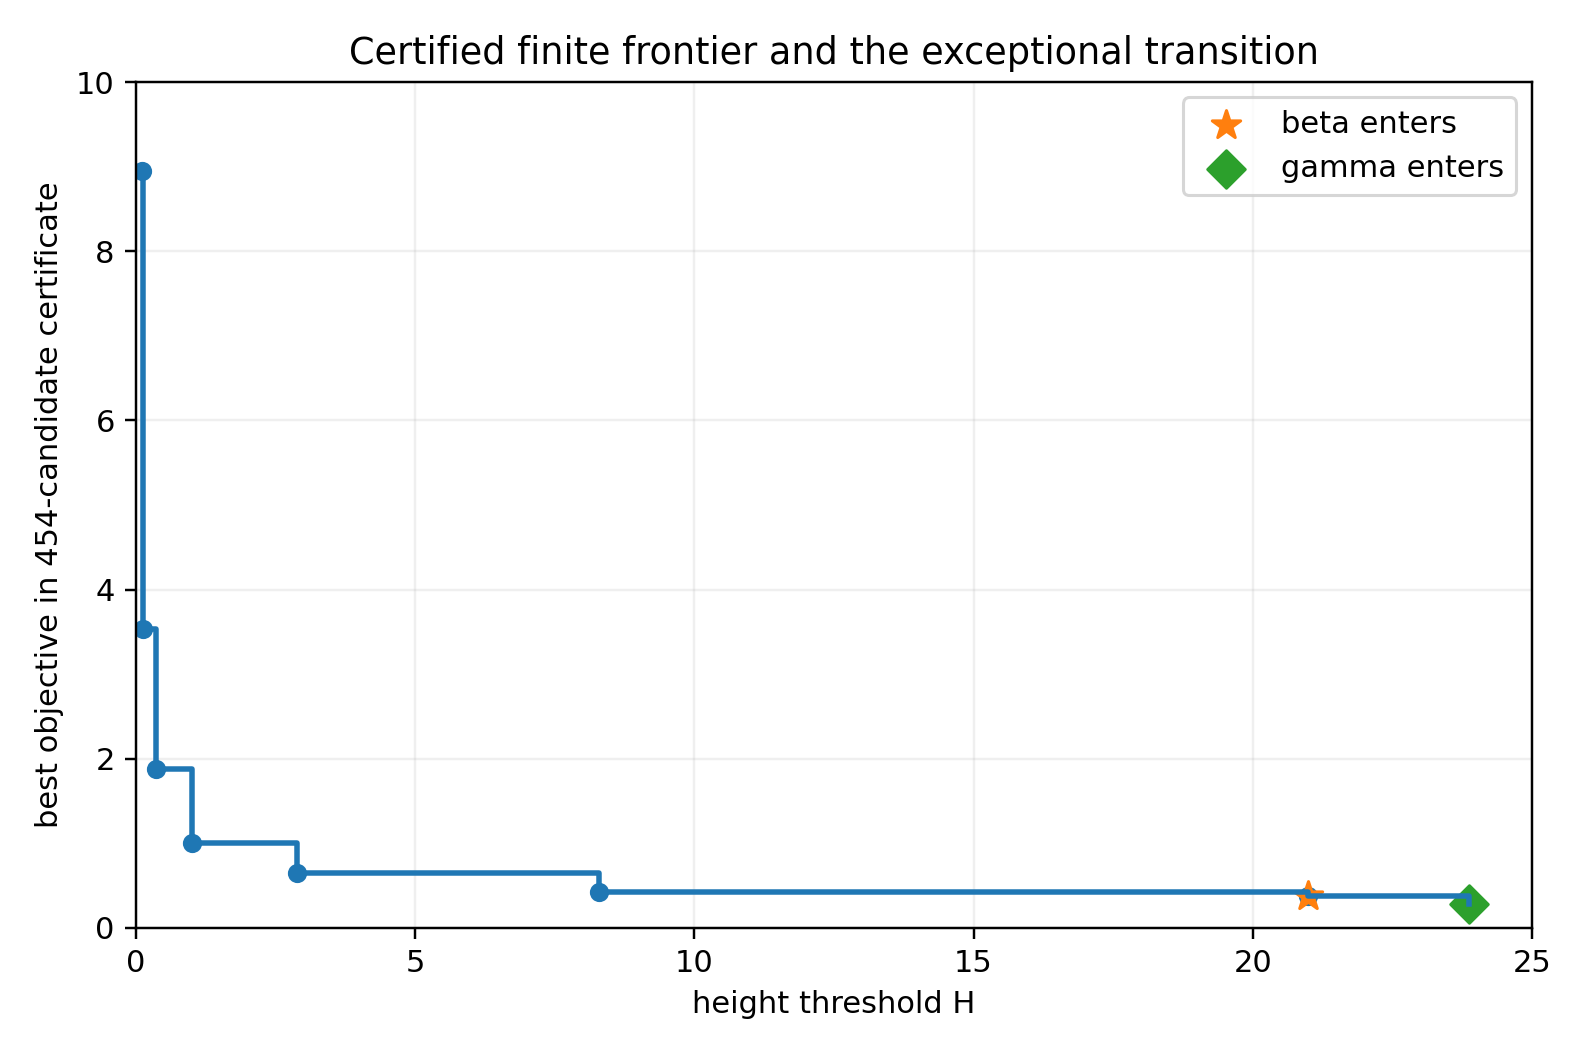
\includegraphics[width=0.84\textwidth]{bounded_frontier.png}
\caption{The record frontier inside the complete 454-triple certificate relevant to \cref{thm:beta}.  The theorem does not infer global behavior outside the certified transition window from this finite plot.}
\label{fig:frontier}
\end{figure}

\section{What is proved, and what remains open}
The results above separate three levels that were previously easy to conflate.

\begin{enumerate}[label=\textbf{\arabic*.},leftmargin=2em]
\item \textbf{Global structural theorem.}  Every optimizer is a unit or a $(\theta-1)$-multiple of a unit; this is \cref{thm:global-reduction}.
\item \textbf{Global exact transition.}  The nonunit $\beta$ is the unique optimizer up to sign on the exact interval $[L,U)$, and $\gamma$ takes over at $U$; this is \cref{thm:beta}.
\item \textbf{Distributional theory.}  Numerical work motivating this project suggests a logarithmic exceptional density near $0.01945222156$ and an oscillatory ordinary sampling law.  Those claims are \emph{not} proved in this release.  A proof still requires a complete analysis of how the two unit-coset layers alternate over all logarithmic heights.
\end{enumerate}

The norm-coset reduction materially narrows the third problem: no other norm layer can create a hidden optimizer.  What remains is a two-lattice switching problem rather than an unrestricted search over all algebraic integers.

\section{Verification protocol}
The release includes a standalone script, \texttt{verify.py}.  Its pass/fail decisions use exact integers and rational numbers only.  The verifier checks:
\begin{itemize}
\item isolation of the three roots of $x^3-3x-1$;
\item the identities defining $\beta$, $\gamma$, and the ramified norm-$3$ layer;
\item the 16-by-16 log-lattice covering certificate, with logarithms bounded by rational series remainders;
\item the inverse-Vandermonde coefficient bounds proving completeness of the 454-triple box;
\item all 454 finite comparisons in \cref{thm:beta}; and
\item the inertness tests modulo $2$, $5$, and $7$ used in the norm gap.
\end{itemize}
The discovery calculations and the verifier are deliberately separated.  A reader can rerun the verifier without trusting the numerical search that originally suggested $\beta$.

\section{Relation to classical cubic-field geometry}
The field in this paper is the $a=0$ member of Shanks' simplest cubic family.  The general family, its units, and its cyclic structure were studied by Shanks \cite{Shanks1974}.  Voronoi reduction, relative minima, and the geometry of cubic ideals give a broad classical framework for understanding special lattice points in cubic fields; a modern treatment is given by Hambleton and Williams \cite{HW2018}.  Fundamental-parallelepiped methods also appear in recent work on indecomposable integers in totally real cubic fields, for example \cite{KalaSgallovaTinkova2025,Tinkova2023}.

The one-sided constrained minimax functional \eqref{eq:M} is not the standard relative-minimum problem.  The present manuscript therefore makes only the claims proved above and does not assert that the general geometric viewpoint is new.  A full novelty assessment would require a more exhaustive comparison with the literature on relative minima, reduction, and inhomogeneous approximation in cubic fields.

\section{Conclusion}
The main obstruction in this project was not finding an unusual candidate; it was proving that the candidate could not be defeated by an algebraic integer outside the search window.  The inverse-Vandermonde argument removes that obstruction for the principal transition, upgrading a finite search into the exact global interval theorem \cref{thm:beta}.  Independently, the log-lattice covering argument and the small-norm arithmetic reduce the entire optimization problem to two multiplicative layers, \cref{thm:global-reduction}.  These results provide a rigorous base from which the remaining density and switching questions can be attacked without hidden norm layers or unverified finite-search assumptions.

\small
\begin{thebibliography}{9}
\bibitem{Shanks1974}
D. Shanks,
\newblock The simplest cubic fields,
\newblock \emph{Mathematics of Computation} \textbf{28} (1974), 1137--1152.
\newblock DOI: 10.1090/S0025-5718-1974-0352049-8.

\bibitem{HW2018}
S. A. Hambleton and H. C. Williams,
\newblock \emph{Cubic Fields with Geometry},
\newblock CMS Books in Mathematics, Springer, 2018.

\bibitem{Tinkova2023}
M. Tinkov\'a,
\newblock Trace and norm of indecomposable integers in cubic orders,
\newblock \emph{Ramanujan Journal} \textbf{61} (2023), 1121--1144.
\newblock DOI: 10.1007/s11139-022-00669-y.

\bibitem{KalaSgallovaTinkova2025}
V. Kala, E. Sgallov\'a, and M. Tinkov\'a,
\newblock Arithmetic of cubic number fields: Jacobi--Perron, Pythagoras, and indecomposables,
\newblock \emph{Journal of Number Theory} \textbf{273} (2025), 37--95.
\newblock DOI: 10.1016/j.jnt.2024.12.001.
\end{thebibliography}

\end{document}
